%% BioMed_Central_Tex_Template_v1.06
%%                                      %
%  bmc_article.tex            ver: 1.06 %
%                                       %

%%IMPORTANT: do not delete the first line of this template
%%It must be present to enable the BMC Submission system to
%%recognise this template!!

%%%%%%%%%%%%%%%%%%%%%%%%%%%%%%%%%%%%%%%%%
%%                                     %%
%%  LaTeX template for BioMed Central  %%
%%     journal article submissions     %%
%%                                     %%
%%          <8 June 2012>              %%
%%                                     %%
%%                                     %%
%%%%%%%%%%%%%%%%%%%%%%%%%%%%%%%%%%%%%%%%%


%%%%%%%%%%%%%%%%%%%%%%%%%%%%%%%%%%%%%%%%%%%%%%%%%%%%%%%%%%%%%%%%%%%%%
%%                                                                 %%
%% For instructions on how to fill out this Tex template           %%
%% document please refer to Readme.html and the instructions for   %%
%% authors page on the biomed central website                      %%
%% http://www.biomedcentral.com/info/authors/                      %%
%%                                                                 %%
%% Please do not use \input{...} to include other tex files.       %%
%% Submit your LaTeX manuscript as one .tex document.              %%
%%                                                                 %%
%% All additional figures and files should be attached             %%
%% separately and not embedded in the \TeX\ document itself.       %%
%%                                                                 %%
%% BioMed Central currently use the MikTex distribution of         %%
%% TeX for Windows) of TeX and LaTeX.  This is available from      %%
%% http://www.miktex.org                                           %%
%%                                                                 %%
%%%%%%%%%%%%%%%%%%%%%%%%%%%%%%%%%%%%%%%%%%%%%%%%%%%%%%%%%%%%%%%%%%%%%

%%% additional documentclass options:
%  [doublespacing]
%  [linenumbers]   - put the line numbers on margins

%%% loading packages, author definitions

%\documentclass[twocolumn]{bmcart}% uncomment this for twocolumn layout and comment line below
\documentclass{bmcart}

%%% Load packages
%\usepackage{amsthm,amsmath}
%\RequirePackage{natbib}
%\RequirePackage[authoryear]{natbib}% uncomment this for author-year bibliography
%\RequirePackage{hyperref}
\PassOptionsToPackage{hyphens}{url}\usepackage{hyperref}
\usepackage[utf8]{inputenc} %unicode support
%\usepackage[applemac]{inputenc} %applemac support if unicode package fails
%\usepackage[latin1]{inputenc} %UNIX support if unicode package fails


%%%%%%%%%%%%%%%%%%%%%%%%%%%%%%%%%%%%%%%%%%%%%%%%%
%%                                             %%
%%  If you wish to display your graphics for   %%
%%  your own use using includegraphic or       %%
%%  includegraphics, then comment out the      %%
%%  following two lines of code.               %%
%%  NB: These line *must* be included when     %%
%%  submitting to BMC.                         %%
%%  All figure files must be submitted as      %%
%%  separate graphics through the BMC          %%
%%  submission process, not included in the    %%
%%  submitted article.                         %%
%%                                             %%
%%%%%%%%%%%%%%%%%%%%%%%%%%%%%%%%%%%%%%%%%%%%%%%%%


%\def\includegraphic{}
%\def\includegraphics{}
\usepackage{graphicx}


%%% Put your definitions there:
\startlocaldefs
\endlocaldefs

\newcommand{\variantSpark}{{\sc VariantSpark}}
\newcommand{\kMeans}{\textit{k}-means}
\newcommand{\ARI}{adjusted Rand index}


%%% Begin ...
\begin{document}

%%% Start of article front matter
\begin{frontmatter}

\begin{fmbox}
\dochead{Research}

%%%%%%%%%%%%%%%%%%%%%%%%%%%%%%%%%%%%%%%%%%%%%%
%%                                          %%
%% Enter the title of your article here     %%
%%                                          %%
%%%%%%%%%%%%%%%%%%%%%%%%%%%%%%%%%%%%%%%%%%%%%%

\title{VariantSpark: Population Scale Clustering of Genotype Information}

%%%%%%%%%%%%%%%%%%%%%%%%%%%%%%%%%%%%%%%%%%%%%%
%%                                          %%
%% Enter the authors here                   %%
%%                                          %%
%% Specify information, if available,       %%
%% in the form:                             %%
%%   <key>={<id1>,<id2>}                    %%
%%   <key>=                                 %%
%% Comment or delete the keys which are     %%
%% not used. Repeat \author command as much %%
%% as required.                             %%
%%                                          %%
%%%%%%%%%%%%%%%%%%%%%%%%%%%%%%%%%%%%%%%%%%%%%%

\author[
   addressref={aff1,aff2},                   % id's of addresses, e.g. {aff1,aff2}
%   corref={aff1},                       % id of corresponding address, if any
%   noteref={n1},                        % id's of article notes, if any
%   email={jane.e.doe@cambridge.co.uk}   % email address
]{\inits{}\fnm{Aidan R.} \snm{O'Brien}}
\author[
   addressref={aff1},
]{\inits{}\fnm{Neil} \snm{Saunders}}
\author[
   addressref={aff3,aff4},
%   email={john.RS.Smith@cambridge.co.uk}
]{\inits{}\fnm{Fabian A.} \snm{Buske}}
\author[
   addressref={aff1},
   email={Denis.Bauer@CSIRO.au}
%   email={john.RS.Smith@cambridge.co.uk}
]{\inits{}\fnm{Denis C.} \snm{Bauer}}
%%%%%%%%%%%%%%%%%%%%%%%%%%%%%%%%%%%%%%%%%%%%%%
%%                                          %%
%% Enter the authors' addresses here        %%
%%                                          %%
%% Repeat \address commands as much as      %%
%% required.                                %%
%%                                          %%
%%%%%%%%%%%%%%%%%%%%%%%%%%%%%%%%%%%%%%%%%%%%%%

\address[id=aff1]{%                           % unique id
  \orgname{CSIRO, Health \& Biosecurity Flagship}, % university, etc
  \street{11 Julius Av},                     %
  \postcode{2113},                                % post or zip code
  \city{Sydney},                              % city
  \cny{Australia}                                    % country
}
\address[id=aff2]{%
  \orgname{School of Biomedical Sciences and Pharmacy, Faculty of Health},
  \postcode{2308},
  \city{Newcastle},
  \cny{Australia}
}
\address[id=aff3]{%
  \orgname{Cancer Epigenetics Program, Cancer Research Division, Kinghorn Cancer Centre, Garvan Institute of Medical Research},
  \street{384 Victoria St},
  \postcode{2010},
  \city{Sydney},
  \cny{Australia}
}
\address[id=aff4]{%
  \orgname{UNSW Medicine, University of New South Wales},
%  \street{384 Victoria St},
  \postcode{2052},
  \city{Sydney},
  \cny{Australia}
}
%%%%%%%%%%%%%%%%%%%%%%%%%%%%%%%%%%%%%%%%%%%%%%
%%                                          %%
%% Enter short notes here                   %%
%%                                          %%
%% Short notes will be after addresses      %%
%% on first page.                           %%
%%                                          %%
%%%%%%%%%%%%%%%%%%%%%%%%%%%%%%%%%%%%%%%%%%%%%%

\begin{artnotes}
%\note{Sample of title note}     % note to the article
\note[id=n1]{Equal contributor} % note, connected to author
\end{artnotes}

\end{fmbox}% comment this for two column layout

%%%%%%%%%%%%%%%%%%%%%%%%%%%%%%%%%%%%%%%%%%%%%%
%%                                          %%
%% The Abstract begins here                 %%
%%                                          %%
%% Please refer to the Instructions for     %%
%% authors on http://www.biomedcentral.com  %%
%% and include the section headings         %%
%% accordingly for your article type.       %%
%%                                          %%
%%%%%%%%%%%%%%%%%%%%%%%%%%%%%%%%%%%%%%%%%%%%%%

\begin{abstractbox}

\begin{abstract} % abstract
\parttitle{Motivation} Genomic information is increasingly used in medical practice giving rise to the need for efficient analysis methodology able to cope with thousands of individuals and millions of variants. The widely used Hadoop MapReduce architecture and associated machine learning library, Mahout, provide the means for tackling computationally challenging tasks. However, many genomic analyses do not fit the Map-Reduce paradigm. 
We therefore utilise the recently developed {\sc Spark} engine, along with its associated machine learning library, MLlib, which offers more flexibility in the parallelisation of population-scale bioinformatics tasks. 
\variantSpark{} provides an interface from MLlib to the standard variant format (VCF), offers seamless genome-wide sampling of variants and provides a pipeline for visualising results. 

\parttitle{Results} To demonstrate the capabilities of \variantSpark, we clustered more than 1,000 individuals with 38 Million variants each to determine the population structure in the dataset. \variantSpark{} is 80\% faster than the {\sc Spark}-based genome clustering approach, {\sc ADAM}, the comparable implementation using Hadoop/Mahout, as well as a {\sc Admixture}, a commonly used tool for determining individual ancestries. It is over 90\% faster than traditional implementations using R and Python.
These benefits of speed, resource consumption and scalability enables \variantSpark{} to open up the usage of advanced, efficient machine learning algorithms to genomic data. 


\parttitle{Availability} The package is written in Scala and available at \url{https://github.com/BauerLab/VariantSpark}.
\end{abstract}

%%%%%%%%%%%%%%%%%%%%%%%%%%%%%%%%%%%%%%%%%%%%%%
%%                                          %%
%% The keywords begin here                  %%
%%                                          %%
%% Put each keyword in separate \kwd{}.     %%
%%                                          %%
%%%%%%%%%%%%%%%%%%%%%%%%%%%%%%%%%%%%%%%%%%%%%%

\begin{keyword}
\kwd{Genotype clustering}
\kwd{SPARK}
\kwd{BigData}
\kwd{1000 Genomes Project}
\kwd{Personal Genome Project}
\kwd{Population structure}
\end{keyword}

% MSC classifications codes, if any
%\begin{keyword}[class=AMS]
%\kwd[Primary ]{}
%\kwd{}
%\kwd[; secondary ]{}
%\end{keyword}

\end{abstractbox}
%
%\end{fmbox}% uncomment this for twcolumn layout

\end{frontmatter}

%%%%%%%%%%%%%%%%%%%%%%%%%%%%%%%%%%%%%%%%%%%%%%
%%                                          %%
%% The Main Body begins here                %%
%%                                          %%
%% Please refer to the instructions for     %%
%% authors on:                              %%
%% http://www.biomedcentral.com/info/authors%%
%% and include the section headings         %%
%% accordingly for your article type.       %%
%%                                          %%
%% See the Results and Discussion section   %%
%% for details on how to create sub-sections%%
%%                                          %%
%% use \cite{...} to cite references        %%
%%  \cite{koon} and                         %%
%%  \cite{oreg,khar,zvai,xjon,schn,pond}    %%
%%  \nocite{smith,marg,hunn,advi,koha,mouse}%%
%%                                          %%
%%%%%%%%%%%%%%%%%%%%%%%%%%%%%%%%%%%%%%%%%%%%%%

%%%%%%%%%%%%%%%%%%%%%%%%% start of article main body
% <put your article body there>

%%%%%%%%%%%%%%%%
%% Background %%
%%
\section*{Background}

Genomic information is increasingly used in medical practice.
A commonly performed task in such applications is grouping individuals based on their genomic profile to identify population association~\cite{Gao2007} or elucidate haplotype involvement in diseases susceptibility~\cite{Laitman2013}.
The commonly used tool is {\sc Admixture}~\cite{Alexander2009}, which performs maximum likelihood estimation of individual ancestries from multilocus SNP genotype datasets.
Due to the decreasing sequencing cost it is now economical to generate studies with sample sizes previously reserved for larger consortia such as the 1000 Genomes Project~\cite{1KG2012} or The Cancer Genome Atlas, TCGA~\cite{TCGA2013}. 
At the same time, whole genome sequencing enables the inclusion of rare or even somatic mutations in the analysis, increasing the feature space by orders of magnitude. This drastic increase in both sample numbers and features per sample requires a massively parallel approach to data processing~\cite{Stein2010}. Traditional parallelisation strategies like MPI/OpenMP or hardware accelerators (GPGPU) cannot scale with variable data sizes at runtime~\cite{ReyesOrtiz2015121} or require purpose-built hardware.
 
Addressing this issue, {\sc Apache Hadoop MapReduce}~\cite{Borthakur2007} transforms data into `key-value pairs' that can then be distributed between multiple nodes across a commodity computer cluster, depending on the size of the problem. 
MapReduce approaches are increasingly being used in bioinformatics (for reviews see~\cite{Zou2013, Qiu2010,Taylor2010}). 
This is especially the case for sequence analysis tasks, such as read mapping~\cite{Schatz2009}, duplicate removal~\cite{Jourdren2012}, and variant calling~\cite{Langmead2009, McKenna2010} as well as Genome Wide Analysis Study based tasks~\cite{Huang2013, Guo2014}. 
Apache also developed a machine learning library, Mahout~\cite{Owen2011}, which allows efficient out-of-the-box analysis to be applied to clinical applications, such as medical health records~\cite{Ko2014}.
Unfortunately, the MapReduce paradigm is not always the optimal solution, specifically for bioinformatics or machine learning applications that require iterative in-memory computation. Specifically, Hadoop is relying extensively on hard disk input-output operations (disk IO), and this can prove to be a bottleneck in processing-speed.

{\sc Apache Spark}~\cite{Zaharia2011} is a more recent compute engine, which overcomes many of Hadoop's limitations. 
One of the main benefits is that it allows programs to cache data in memory; potentially eliminating, or at least reducing, the bottleneck of disk IO. 
When utilising caching, Apache claim {\sc Spark} to be up to 100x faster than Hadoop. 
Although {\sc Spark} allows MapReduce-like programs, it does not require programs to exactly model the MapReduce paradigm, which in turn allows more flexible software design. 
Recognising the capability, Wiewi{\'o}rka {\it et al.}~\cite{Wiewiorka2014} developed {\sc SparkSeq} for high-throughput sequence data analysis and the Big Data Genomics (BDG) group recently demonstrated the strength of {\sc Spark} in a genomic clustering application using {\sc ADAM}, a set of formats and APIs as well as processing stage implementations for genomic data~\cite{Massie2013}. 
While the speedup of {\sc ADAM} over traditional methods was impressive (50 fold speedup), being limited by constraints within this general genomics framework hampered performance. 

We hence developed a purpose-built application in {\sc Spark} to perform genomic clustering of individuals. 
We utilise {\sc Spark}'s machine learning library, \mbox{MLlib}, and provide an interface to the standard variant data format, Variant Call Format (VCF)~\cite{1KG2012}, which opens up the application of MLlib's different machine learning algorithms to a wide range of genotype-based analysis tasks. 

To demonstrate \variantSpark's capability, we cluster variant datasets from the 1000 Genomes Project~\cite{1KG2012} to determine population structure using the \kMeans{} clustering algorithm available in MLlib. 
In the first section we benchmark \variantSpark's performance and accuracy against {\sc ADAM} and a Hadoop Mahout implementation as well as more traditional methods (R, Python) and the purpose-build tool {\sc Admixture}~\cite{Alexander2009}. % limiting the used data to chromosome 22.
In the second section we discuss the pipeline for visualising the resulting cluster.
In section three we demonstrate \variantSpark's full capacity by seamlessly scaling from 20\% to 100\% of the human genome.
In the last section we replicate the analysis by using 478 genomes from the Personal Genome Project~\cite{Lunshof2013}.


\section*{Results and discussions}

\subsection*{{\sc Spark} enables faster clustering of individuals compared to traditional methods}

In this section we compare the time required to cluster individuals based on genomic variants using \variantSpark{} against {\sc ADAM} as well as the more traditional approaches using Hadoop (and Mahout), Python and R. 
We limit the genomic variants to only chromosome 22 as the traditional approaches have substantially larger memory consumption, rendering a whole-genome input infeasible.
Furthermore, we perform the comparisons on a single virtual machine to ensure the six different approaches have access to the same resources.
We use \kMeans{} clustering algorithms in the respective implementations, which require the VCF input files to be pre-processed (see methods). 
The state-of-the-art tool, {\sc Admixture}, also requires a pre-processing step from VCF to PED format, which we performed using GATK~\cite{McKenna2010}.
We therefore compare the time required for the pre-processing step, as well as for \kMeans{} clustering.

As shown in Table 1, pre-processing the data is fastest in \variantSpark{}, requiring 3 minutes. %2mins and 58secs. %178s 
This is almost 80\% faster than both the {\sc ADAM} implementation (13 minutes) %(12min and 48secs) %768s
and our Hadoop implementation (14 minutes). %(14min and 22secs). %862s
Unlike \variantSpark{} and our Hadoop implementation, the {\sc ADAM} framework cannot process the VCF files directly but requires them to be converted into a binary {\sc ADAM} file format. 
Although this additional pre-processing step is only required once for each input file, it uses an additional 13 minutes, %13mins and 13secs, %793s
rendering our approach almost an order of magnitude faster (see Figure 1).
R and Python are also slower at pre-processing, taking 67 minutes and 92 minutes, respectively. 
This increased pre-processing time is due to the standard Python and R implementations not natively supporting multithreading, while \variantSpark{}, {\sc ADAM} and Hadoop can use the eight available cores.
The GATK-based VCF to PED conversion for {\sc Admixture} is also slower with over 10 minutes. 

Clustering the samples is also fastest in \variantSpark{} (1min and 20secs, see Table 1), despite \variantSpark{} and {\sc ADAM} both using {\sc Spark}'s MLlib \kMeans{} implementation. % 80
We attribute the 30\% speedup over {\sc ADAM} (1min and 52secs) to \variantSpark{} converting the VCF files to sparse vectors, whereas {\sc ADAM} creates dense vectors, which are less memory efficient. %
Multithreading \kMeans{} clustering is natively supported by both R and Python, we are therefore able to utilise eight cores. 
Despite this, both are an order of magnitude slower than \variantSpark{} and {\sc ADAM}, with Python requiring 11 minutes  and R requiring 8 minutes. %11and 29secs 7mins and 25secs
{\sc Admixture} is also slower with a runtime of just over 8 minutes. 
Our Hadoop implementation performs the worst with 14 minutes, showcasing the limitations of the Hadoop engine for iterative algorithms such as \kMeans{}. % 863 14mins and 23secs
Hadoop writes the entire output of each \kMeans{} iteration to disk. This feature was designed to ensure scalability but here substantially increases the runtime as disk IO becomes the limiting factor for this small dataset (chromosome 22).
Python and R store the output from each iteration in memory, thereby eliminating the IO bottleneck, but without being able to utilise the disk they are limited to datasets that fit into memory.
{\sc Spark} overcomes both limitations by performing in-memory caching for each executor, which eliminates the disk IO bottleneck on smaller datasets, while maintaining scalability to larger datasets by spilling data that exceeds memory availability to disk.

We also investigate the cluster quality for the five different methods by comparing the annotated super-population label (AMR, AFR, EAS, SAS) for each individual in the 1000 Genomes data to the assigned label from the clustering allowing four clusters. 
For this comparison, we use the \ARI{} (ARI) metric, which returns a value between -1 (independent labelings) and 1 (perfect match)~\cite{Hubert1985}.

Using chromosome 22, each of the algorithms resulted in an ARI of 0.84, confirming that the speed-up in {\sc Spark} is not at the cost of quality.
The state-of-the-art tool, {\sc Admixture}, returns a low ARI of 0.25. It should be noted that {\sc Admixture}'s underlying statistical model does not take linkage disequilibrium (LD) into account. 
Therefore removing variants with high LD may result in higher accuracy. 
We can substantially improve the accuracy to a perfect classification (ARI=1.0) by removing the fourth super-population, AMR (American). 
This is due to the majority of AMR individuals being placed in the same group as Europeans, likely reflecting their migrational backgrounds. 
Only a minority of AMR individuals form an independent group, likely comprising of genetic information otherwise not captured by the 26 sub-populations of the 1000 genomes project.
This indicates that although allelic differences exist between populations, "genetic diversity is distributed on a continuum"~\cite{Pugach2015}.

\subsection*{Graph visualisation}
\variantSpark{} supports visualisation of the resulting population clusters by generating a file that can be loaded into {\sc Gephi}~\cite{ICWSM09154}.
Figure 3 visualises the clusters generated by \variantSpark{} from the 1000 Genomes Project data. 
As discussed in the previous section, three of the four clusters (super-populations AFR, EAS and AMR) are relatively homogeneous; the fourth is more mixed and 
consists predominantly of individuals labelled EUR and AMR providing a visual representation of the ARI of 0.84.


\subsection*{\variantSpark{} enables genome wide sampling of variants to improve clustering quality}
Although we have demonstrated the advantages of \variantSpark{} over traditional methods on small datasets, such as individual chromosomes, the main advantage of {\sc Spark} is its ability to process datasets that exceed memory limits.
To demonstrate this scalability, we increase the number of variants used in the clustering from the initial 494,328 on chromosome 22 to 38,219,238 including all variants in the genome.

We run this comparison on our in-house Hadoop cluster using 40 cores.
Pre-processing the VCF files takes approximately 12, 19, 27 and 40 minutes for 20, 40, 60 and 100 percent of the genome, respectively (see Table 2).
In each case, the memory required does not exceed a modest 2GB per executor, even for the complete genome. 
Clustering the data takes 70 minutes, 139 minutes, 213 minutes and 884 mins, respectively.
For clustering, the memory requirements increase approximately linearly to 24GB per executor (see Figure 1). 
The increase in memory is due to more distance measurements between variants and \kMeans{} centroids being created, which MLlib stores as dense vectors. 
While \kMeans{} clustering can scale to 100\% of the genome, machine learning algorithms that can deal with sparse vectors would potentially be able to scale much further, for example process more alleles.

We do not observe an increase in cluster accuracy when providing variants from all chromosomes, indicating that current practice of clustering based on a subset of the genome is sufficient to define the existing population boundaries for populations with large genetic distance~\cite{Pugach2015}.

%To further demonstrate the scalability of \variantSpark{}, we also cluster the larger 1000 Genomes Project phase 3 VCF files. Although \kMeans{} clustering completes successfully on this dataset,
%it takes over 27 hours (see Table 2) due to more than twice the number of individuals, and hence more variants. For comparison, the uncompressed size of the phase 3 files is 770GB vs the 161GB of the phase 1 dataset.
To further demonstrate the scalability of \variantSpark{}, we also cluster the 1000 Genomes Project phase 3 data, which contains 3000 individuals from 5 super-populations and as a result has over 80 Million variants. 
The uncompressed size of the phase 3 files is 770GB compared to the 161GB of the phase 1 dataset.
\variantSpark{} successfully completes the clustering in just 27 hours (see Table 2) with an ARI of 0.82. 



\subsection*{Determining the population structure of the Personal Genome Project}
To demonstrate the versatility of \variantSpark{} we also process and cluster individuals from the Personal Genomics Project (PGP). The PGP is open to the public for individuals to submit their genomic sequence along with any metadata, such as diseases or clinical features~\cite{Lunshof2013}. 
We obtain and curate the data (see methods) resulting in 985,790 variants from 478 individuals.

We cluster the individuals allowing five clusters and compare the assigned labels to the same number of self-reported `Race/ethnicity' labels (`White', `Hispanic or Latino', `Asian', `Black or African American' and `American Indian').
The observed ARI is negative, indicating the clustering is random. 
This poor result may be due to the labels being too broad and not accurately reflecting genetic diversity. For example, the `White' label includes individuals with grandparents from United States, Syria, Arab Republic, or Bulgaria, amongst others. 
The dataset is also very one-sided with 433 out of the 478 (over 90\%) of the individuals being classified as white, even though geographical location of their grandparents are very diverse.
We therefore only include individuals where all grandparents were reported to be from the same country leaving 35 individuals from 22 different countries, which we group into their approximate super-populations (see Supplemental Table 1). 
Clustering these individuals results in an ARI of 0.45. 

Although we see an increase in cluster-accuracy when removing individuals with a mixed background and operating at super-population level, the clustering is not as precise as on the carefully curated and characterised individuals from the 1000 Genomes Project.
This is especially the case since 65\% are `White' Americans, which formed the group most difficult to cluster in the 1000 Genomes Project data.

This highlights the issue for clinical application where ancestry influences treatment (e.g. HLA allele genotyping from SNP information~\cite{Zheng2014}) and accurate population association may not be known for patients with diverse migrational background.
As noted by Patterson et al ~\cite{Patterson2006}, more markers are needed for populations with low genetic divergence. 
It is hence likely that higher density genotyping (e.g. from genome sequencing) would help in elucidating population structure in this dataset, which demonstrates the need for fast whole-genome approaches. 
Unfortunately, this hypothesis can no not be tested as whole genome information is not available for these individuals. 




\section*{Conclusions}

%\variantSpark{} performs clustering on VCF files with over 1000 individuals and 40 million variants in under 15 hours using minimal memory (24GB). 
\variantSpark{} performs clustering on VCF files with over 3000 individuals and 80 million variants in 27 hours using minimal memory (24GB). 
\variantSpark{} supports random genome-wide sampling of variants allowing faster clustering for well characterised cohorts where 20\% of the genome is sufficient. 
On the benchmarking dataset, it outperforms {\sc ADAM} by almost an order of magnitude (4 vs 28 minutes) by processing VCF files directly and storing the information in sparse vectors. % 258 vs 1673 
\variantSpark{} utilises {\sc Spark}, which allows for in-memory caching and hence performs 85\% faster than Hadoop (29 min).
\variantSpark{} scales to data sizes that are not feasible to process using R or Python due their requirement to load the whole dataset into memory. 
But even on the small benchmarking dataset, \variantSpark{}'s novel parallelisation approach is faster than traditional multithreading with 94\% speedup over R (75 min), and 95\% over Python (103 min).
\variantSpark{} is also superior in performance and accuracy over the current state-of-the-art tool for individual ancestries determination, {\sc Admixture}.
These benefits of speed, resource consumption and scalability allows \variantSpark{} to be the interface for applying other machine learning tools from MlLib to genomic data. 
Utilising MLlib as well as Spark.ML will enable supervised machine learning applications to e.g. identify variants that jointly interact with phenotypes as well as include electronic health record in addition to the genomic feature vector to e.g. capture medical history as well as predispositions for diagnosis and treatment decisions. 




\section*{Materials and methods}
\subsection*{Computational resources}
We completed the Chromosome 22 comparisons on a virtual machine (VM) hosted on Microsoft Azure. This VM is an A7 Linux instance with 8 cores, 56GB
memory running Ubuntu. 
For the whole-genome clustering, we used our in-house Hadoop cluster with Hadoop 2.5.0, managed by cloudera's CDH 5. We use Spark 1.3.1. This 13 node
cluster has a total of 416 cores and 1.22TB memory.


\subsection*{Datasets}
We use the 22 autosomes from the 1000 Genomes Project phase 1 dataset. This dataset contains variants from 1092 individuals, across 38,219,238 alleles.
For the smaller dataset, we use the variants from chromosome 22, with 494,328 alleles.
The individuals from these datasets are distributed across four super populations, African (AFR), Mixed American (AMR), East Asian (EAS) and European (EUR).
We also cluster the Phase 3 dataset, which contains variants from 2535 individuals, across 81,271,745 variants. As well as the above for super populations, this
dataset also includes South Asian (SAS).



\subsection*{VariantSpark Implementation}
To cluster individuals from a VCF file, we initially need to pre-process the variants to feature vectors.
In \variantSpark{} we read in VCF files as text files, to a Resilient Distributed Dataset (RDD). RDDs allow us to process the files, line-by-line, in parallel.

We parse each line as tab-separated values, and store these the values from each line in an array.

For each array, we use Spark's `zip' function to `zip' each value with it's heading (Sample name) from the VCF file. Now each array element is a
key-value pair (KVP) of the previous value and its heading. For the KVPs that contain an allele as the value, the key (derived from the heading) is
the Individual ID (see Figure 2, Spark step 1).

For each array, we remove any KVPs that represent data other than alleles (such as the genomic location). With the remaining KVPs, which all
represent alleles, we apply a function to convert these from the strings found in VCF files (i.e. `0\textbar{}1'), to doubles, where the double is the
Hamming distance to the reference. I.e. a 1 represents a heterozygous variant, 2, a homozygous variant, and 0, no variant. Because we will
eventually be converting this data to sparse vectors, we remove any KVPs with a value of 0 (i.e. no variant).

At this stage, we can optionally filter variants that don't match a specific criteria. For the Phase 3 dataset, we exclude rare variants that are present in
only one individual. Because each array now only contains variants (rather than every allele), we can simply drop arrays with a length of one, as the length
of each array is equal to the number of individuals who have a variant at that allele.

Now that the dataset only contains alleles we are interested in, we `zip' each array with a unique sequential index (allele ID). This index will serve
as identifier for each allele (and keep the genome loci order) (step 2).

Although we now have the data we require, the variants are stored in arrays of alleles, whereas we require the data to be transposed into arrays of individuals.
To facilitate the grouping of variants by individuals, we use `flatMap' to flatten out the arrays into a collection of KVPs, where the key is the individual ID, and the
value is a tuple of the variant ID and the variant.

We can now group these KVPs by their key (individual ID) and save them to sparse vectors (step 4).


\subsection*{{\sc ADAM} Implementation}
For our {\sc ADAM} comparison, we followed the {\sc ADAM} implementation from (\url{http://bdgenomics.org/blog/2015/02/02/scalable-genomes-clustering-with-adam-and-spark/}).

\subsection*{Hadoop Implementation}
Our Hadoop implementation is based on the MapReduce model, which utilises KVPs, similarly to \variantSpark{}.
As we need a unique range of identifiers for alleles (in the smallest range possible), we need to run an initial MapReduce task to index the lines. This is comparable (however, more verbose) to the `zip' operation in \variantSpark{}.
The second MapReduce task does the bulk of the work and is visualised in Figure 2. The Map stage (step 1) begins by creating KVPs from the VCF file. For each KVP, the key is a tuple of a primary and secondary key, where the primary key is the individual ID and the secondary key is the allele ID. The value for each KVP is the variant.
The primary key ensures that KVPs for each individual are distributed to the same node during the MapReduce shuffle stage. After being distributed, the KVPs for each individual are sorted by their secondary key.
Now that the KVPs for each individual are physically located on the same hardware, the Reduce stage (step 2) can efficiently create a sparse vector for each individual from these KVPs. 

\subsection*{R Implementation}
For our R implementation, we read in a VCF file using {\sc read.table}, and then convert the resulting table to a matrix ({\sc vcfMatrix} with {\sc as.data.frame.matrix}.
%TODO VariantAnnotation reads in the file quicker but causes issue down the track so overall read.table is faster, right ? - can you add this explanation to the supplementary material.
In the supplementary material we benchmark this faster approach against reading the VCF file in using the `VariantAnnotation' package.
We remove the first 9 columns which leaves us with just the variants. As with our \variantSpark{} pre-processing, we convert the strings that represent each allele to a numeric value.
We then transpose the matrix with {\sc t(vcfMatrix)}, which results in a data-structure where each row represents an individual. We convert the matrix to a {\sc big.matrix} object,
as required by the \kMeans{} algorithm from the `biganalytics' package (\url{https://cran.r-project.org/web/packages/biganalytics/index.html}), and then call {\sc bigkmeans} with
the {\sc big.matrix} object and the required number of clusters as arguments.

\subsection*{Python Implementation}
Our Python implementation reads in lines from a VCF file as tab-separated values using {\sc DataFrame.from\textunderscore{}csv}, and stores the data in a pandas DataFrame (\url{http://pandas.pydata.org}). The column headings are the individual IDs and the row headings are the allele locations.
We the first 9 columns and convert the remaining allele strings to numeric values.
We convert the DataFrame to a matrix with {\sc .as\textunderscore{}matrix()} and cluster the matrix using sci-kit learn (\url{http://scikit-learn.org/stable/}).

\subsection*{{\sc Admixture} Implementation}
We use Genome Analysis Toolkit ({\sc -T VariantsToBinaryPed})~\cite{McKenna2010} to convert the variants from VCF, and a 1000 Genomes Project supplied .ped file, to a binary PLINK (.bed), binary marker information file (.bim) and pedigree stub file (.fam).
These three files are used as input to {\sc Admixture}, with default options and $K$ (the number of ancestral populations) set to 4.

\subsection*{Personal Genome Project Data}
Genome data was downloaded from the Personal Genome Project Data (PGP) website (\url{https://my.pgp-hms.org/public_genetic_data}). Genotype data from 23andMe microarray platforms was sorted by genome 
build. Shell scripts were written to convert NCBI build 36 files to BED format, update to build 37 using UCSC liftOver (\url{https://genome.ucsc.edu/cgi-bin/hgLiftOver}) and 
then convert back to 23andMe format. The 23andMe files were then converted to VCF format using code obtained from the Broad Institute (\url{http://apol1.blogspot.com.au/2013/08/impute-apoe-and-apol1-with-23andme.html}). 
Where individuals had genotype data for both genome builds 36 and 37, only the latter was used. Finally, individual VCF files were combined for clustering into one 
file using VCFtools \cite{Danecek2011Variant}.


%%%%%%%%%%%%%%%%%%%%%%%%%%%%%%%%%%%%%%%%%%%%%%
%%                                          %%
%% Backmatter begins here                   %%
%%                                          %%
%%%%%%%%%%%%%%%%%%%%%%%%%%%%%%%%%%%%%%%%%%%%%%

\begin{backmatter}

\section*{Competing interests}
  The authors declare that they have no competing interests.

\section*{Author's contributions}
    DCB and FAB designed the overall study. ARO implemented \variantSpark\ and conducted the comparison. NS obtained the PGP data and generated the graph.
    All authors contributed to the writing of the document. 

\section*{Acknowledgements}
  A.R.O was funded by the NSW Cancer Institute Big Data Big Impact schema, F.A.B by the National Health and Medical Research Council [1051757] and both D.C.B and N.S by Commonwealth Scientific and Industrial Research Organisation's Transformational Capability Platform, Science and Industry Endowment Fund and Information Management and Technology Services. The computation on Azure was funded by Microsoft Azure Research Award. 
The authors would like to thank Piotr Szul and Gareth Williams for their help with setting up Hadoop on the HPC system.

%%%%%%%%%%%%%%%%%%%%%%%%%%%%%%%%%%%%%%%%%%%%%%%%%%%%%%%%%%%%%
%%                  The Bibliography                       %%
%%                                                         %%
%%  Bmc_mathpys.bst  will be used to                       %%
%%  create a .BBL file for submission.                     %%
%%  After submission of the .TEX file,                     %%
%%  you will be prompted to submit your .BBL file.         %%
%%                                                         %%
%%                                                         %%
%%  Note that the displayed Bibliography will not          %%
%%  necessarily be rendered by Latex exactly as specified  %%
%%  in the online Instructions for Authors.                %%
%%                                                         %%
%%%%%%%%%%%%%%%%%%%%%%%%%%%%%%%%%%%%%%%%%%%%%%%%%%%%%%%%%%%%%

% if your bibliography is in bibtex format, use those commands:
\bibliographystyle{bmc-mathphys} % Style BST file (bmc-mathphys, vancouver, spbasic).
\bibliography{genotypeClustering}      % Bibliography file (usually '*.bib' )
% for author-year bibliography (bmc-mathphys or spbasic)
% a) write to bib file (bmc-mathphys only)
% @settings{label, options="nameyear"}
% b) uncomment next line
%\nocite{label}

% or include bibliography directly:
% \begin{thebibliography}
% \bibitem{b1}
% \end{thebibliography}

%%%%%%%%%%%%%%%%%%%%%%%%%%%%%%%%%%%
%%                               %%
%% Figures                       %%
%%                               %%
%% NB: this is for captions and  %%
%% Titles. All graphics must be  %%
%% submitted separately and NOT  %%
%% included in the Tex document  %%
%%                               %%
%%%%%%%%%%%%%%%%%%%%%%%%%%%%%%%%%%%

%%
%% Do not use \listoffigures as most will included as separate files

\section*{Figures}
  \begin{figure}[h!]
  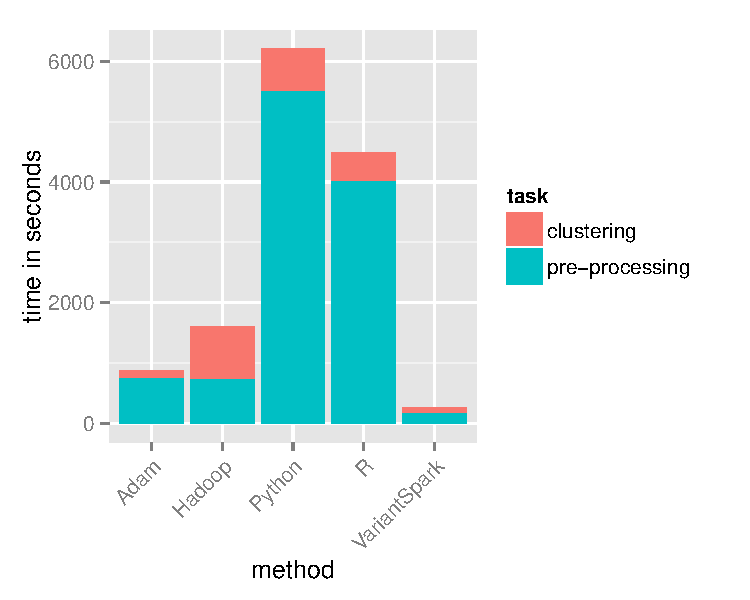
\includegraphics[type=pdf,ext=.pdf,read=.pdf, scale=0.45]{images/Resources}
  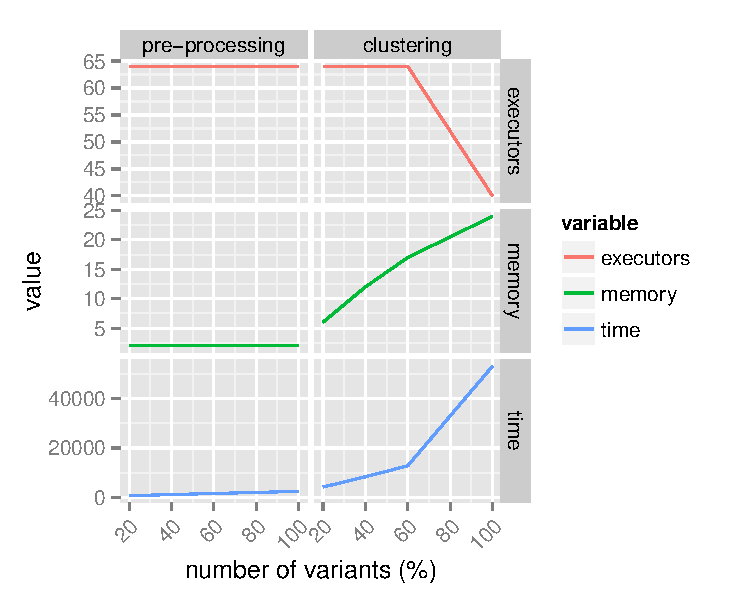
\includegraphics[type=pdf,ext=.pdf,read=.pdf, scale=0.45]{images/Scaling}
  \caption{\csentence{Comparison of method and genome-wide scaling experiment.}
      {\bf Left} Runtime for clustering variants from chromosome 22 is given in seconds with 32 GB of memory on 8 threads (except for the pre-processing in R and Python where this was not supported). 
      {\bf Right} Scaling from 20\% to 100\% of variants in the genome with maximal number of executors and lowest possible memory assignment.}
      \end{figure}

\begin{figure}[h!]
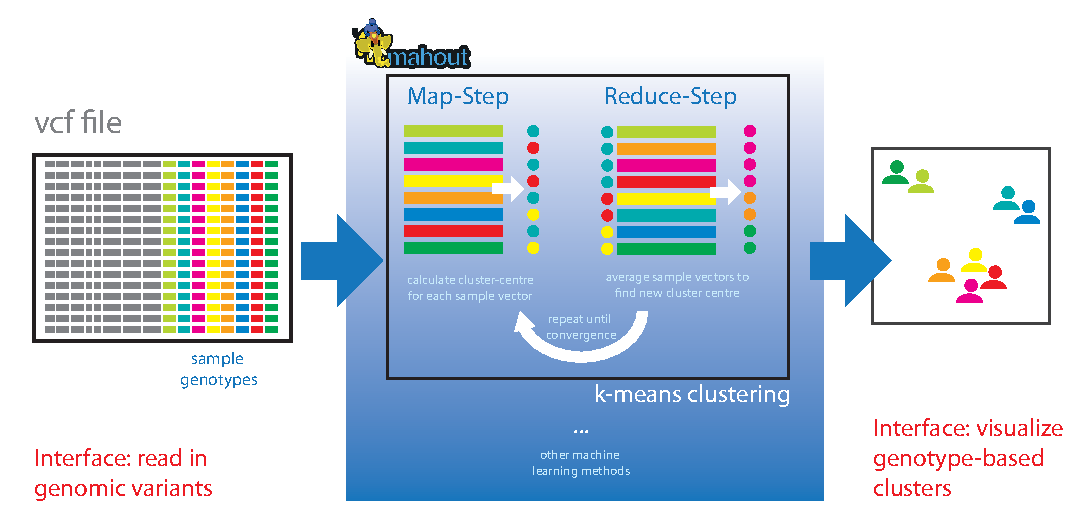
\includegraphics[type=pdf,ext=.pdf,read=.pdf, scale=0.25]{signature}
\caption{\csentence{Schematic overview of VariantSpark}. The image shows the flow from the input VCF file to the machine learning library and onto the visualization. It highlights the differences between the Hadoop and Spark implementations for converting data in VCF format to a data structure readable by Mahout and MLlib, respectively.}
%  \caption{\csentence{Schematic of the Hadoop and Spark implementation.} The image shows the conceptual differences in the steps necessary to convert variants in VCF to a data structure readable by Mahout and MLlib, respectively.}
      \end{figure}

\begin{figure}[h!]
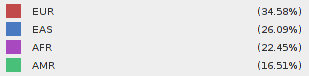
\includegraphics[type=pdf,ext=.pdf,read=.pdf, scale=0.40]{chr22-k4-gephi-legend}
  \caption{\csentence{Visualisation of \variantSpark{} predicted clusters.} The figure shows the four clusters predicted for the 1000 Genomes data. Individuals from the super-populations AFR, AMR and EAS are accurately grouped into distinct clusters. The fourth cluster contains predominantly EUR + AMR individuals potentially accurately reflecting migrational backgrounds.}
%  \caption{\csentence{Visualisation of \variantSpark{} predicted clusters.} Individuals from the 1000 Genomes project are clustered effectively by super-populations AFR, AMR and EAS; a fourth cluster is predominantly EUR + AMR.}
      \end{figure}

%%%%%%%%%%%%%%%%%%%%%%%%%%%%%%%%%%%
%%                               %%
%% Tables                        %%
%%                               %%
%%%%%%%%%%%%%%%%%%%%%%%%%%%%%%%%%%%

%% Use of \listoftables is discouraged.
%%
\section*{Tables}
\label{fivewaycomparison}
\begin{table}[h!]
\caption{The resource consumption of the six compared methods as well as the accuracy measured as \ARI{} on chromosome 22.}
      \begin{tabular}{|c|ccc|ccc|c|c|}
        \hline
           Tool &  \multicolumn{3}{ c |}{Pre-processing} & \multicolumn{3}{ c |}{Clustering} & Accuracy \\
& threads & memory & time  &threads & memory & time  & \\
  \hline
\variantSpark{}	& 8	& 32	& 2min 58sec	& 8	& 32	& 1min 20sec	& 0.84	\\ 
{\sc ADAM}		& 8	& 32	& 12min 48sec	& 8	& 32	& 1min 52sec	& 0.84	\\
Hadoop		& 8	& 32	& 14min 22sec	& 8	& 32	& 14min 23sec	& 0.84	\\
R			& 1	& 32	& 34min 30sec	& 8	& 32	& 7min 25sec	& 0.84	\\
Python		& 1	& 32	& 92min		& 8	& 32	& 11min 29sec	& 0.84	\\
{\sc Admixture}	& 1	& 32	& 10min 8sec	& 8	& 32 & 8min 19sec	& 0.25	\\
  \hline
      \end{tabular}
\end{table}

\label{scalingcomparison}
\begin{table}[h!]
\caption{The resources consumption on different subsets of the entire autosome (chromosomes 1-22). Memory specified is the memory allocated to each executor.}
      \begin{tabular}{|c|ccc|ccc|c|c|}
        \hline
           Portion &  \multicolumn{3}{ c |}{Pre-processing} & \multicolumn{3}{ c |}{Clustering}  \\
& executors & memory & time  & executors & memory & time \\
  \hline
20\%		& 64	& 2	& 11min 53sec	& 64	& 6	& 1hr 10min	\\
40\%		& 64	& 2	& 19min 9sec	& 64	& 12	& 2hr 19min	\\
60\%		& 64	& 2	& 26min 34sec	& 64	& 17	& 3hr 33min	\\
100\%	& 64	& 2	& 40min 48sec	& 40	& 24	& 14hr 44min	\\
???\%	& 64 & 2	& ??min ??sec	& 40 & 24	& 27hr 46min	\\
  \hline
      \end{tabular}
\end{table}



%%%%%%%%%%%%%%%%%%%%%%%%%%%%%%%%%%%
%%                               %%
%% Additional Files              %%
%%                               %%
%%%%%%%%%%%%%%%%%%%%%%%%%%%%%%%%%%%

\section*{Additional Files}
  \subsection*{Additional file 1 --- PGP population labels}
    Conversion map self-reported descriptive population labels to super-population labels.



\end{backmatter}
\end{document}
